% !TEX root = ccsn.tex
\section{Methods description}
\label{methods}

In this section, we outline a strategy for estimating the time evolution of the
ratio $r=M_{\rm PNS}/R_{\rm PNS}^2$ (in units of solar mass and km) from the observation of the $\mbox{}^2g_2$
oscillation mode in the GW detector data.
An integral part of this strategy is the universal relations that relate the
characteristic frequency of the PNS oscillation $f$, $g$ and $p$ modes with the mass
and the radius of the PNS, the shock radius and the total mass inside the shock as
demonstrated in \cite{Torres:2019b}.

To build the model of the ratio $r$ as a function of the frequency $f$ we use the 
spherically symetric (1D) simulations of the {\it model set}. Figure~\ref{fig:LMVAR}
shows the data for the $25$ numerical simulations. As identified by \cite{Torres:2019b}, the only systematic
deviation from a single universal relation is the numerical code used in the simulations. 
To avoid any systematic effect, we only use the $18$ simulations performed with the {\sc AENUS-ALCAR}
code, which is the same code that was used in our test set.
%The consequences of this choice are discussed in the conclusions.
Using this data, we parametrize the discretized ratio $r_i$ with a cubic polynomial
regression with heteroscedastic errors
%Here we are using the data from \textcolor{red}{only {\sc AENUS-ALCAR} or both?, maybe colour-code the two groups of data points } to fit a cubic polyn

\begin{equation}
\label{eq:model1}
r_i=\beta_1 f_i + \beta_2 f_i^2 +\beta_3 f_i^3 + \epsilon_i
\end{equation}
where $\epsilon_i$ are assumed to be independent zero-mean Gaussian errors with
variances $\sigma_i^2$ that increase with frequency $f_i$. The model for frequency-dependent
variances is
\begin{equation}
\log \sigma_i=\alpha_0+ \alpha_1 f_i + \alpha_2 f_i^2 + \delta_i
\end{equation}
with independent and identically zero-mean Gaussian errors $\delta_i$. The R-package \texttt{lmvar}
\cite{lmvar:2019} that implements a maximum likelihood approach was used to fit the model.

The best fitting model amongst polynomials of degree 1, 2, and 3  was chosen according to
the Aikaike information criterion with coefficients given in Table \ref{tab:model}, which is actually the model defined in \eqref{eq:model1}.  The data and fit of the model including 95\% confidence bands are displayed in
Figure~\ref{fig:LMVAR}.

%\begin{equation}\label{eq:universal}
%r_i = \beta_1 f_i + \beta_3 f_i^3 + \epsilon_i
%\end{equation}

%The best-fitting model achieves a coefficient of determination of $R^2=0.9812$.
%The data and fit of the model including 95\% confidence bands are displayed in
%Figure~\ref{fig:LMVAR}.

\begin{table}[h]
%  \begin{tabular}{lll}
%    \hline
%    Coefficient & Estimate & standard error \\
%    \hline
%    $\beta_1$   & $6.09 \times 10^{-7}$ & $1.75 \times 10^{-8}$ \\
%    $\beta_3$   & $6.24 \times 10^{-13}$ & $8.79 \times 10^{-15}$ \\
%    \hline
%  \end{tabular}

  \begin{tabular}{crr}
    \hline
    Coefficient & \multicolumn{1}{c}{Estimate} & Standard error \\
    \hline
   $\beta_1$  &  $ 1.00 \times 10^{-06}$ & $2.12 \times 10^{-08}$ \\   
   $\beta_2$  &  $-8.22 \times 10^{-10}$ & $5.00 \times 10^{-11}$ \\
   $\beta_3$  &  $ 1.01 \times 10^{-12}$ & $2.70 \times 10^{-14}$ \\
   $\alpha_0$ &  $-1.02 \times 10^{+01}$ & $6.80 \times 10^{-02}$ \\
   $\alpha_1$ &  $ 7.24 \times 10^{-04}$ & $1.56 \times 10^{-04}$ \\
   $\alpha_2$ &  $ 6.23 \times 10^{-07}$ & $8.15 \times 10^{-08}$ \\   
    \hline
  \end{tabular}
\caption{Estimate and standard error of the coefficients of the best fit model describing the ratio $r=M_{\rm PNS}/R_{\rm PNS}^2$ as function of the frequency of the $\mbox{}^2g_2$ mode.}\label{tab:model}
\end{table}

\begin{figure}
 \centering
 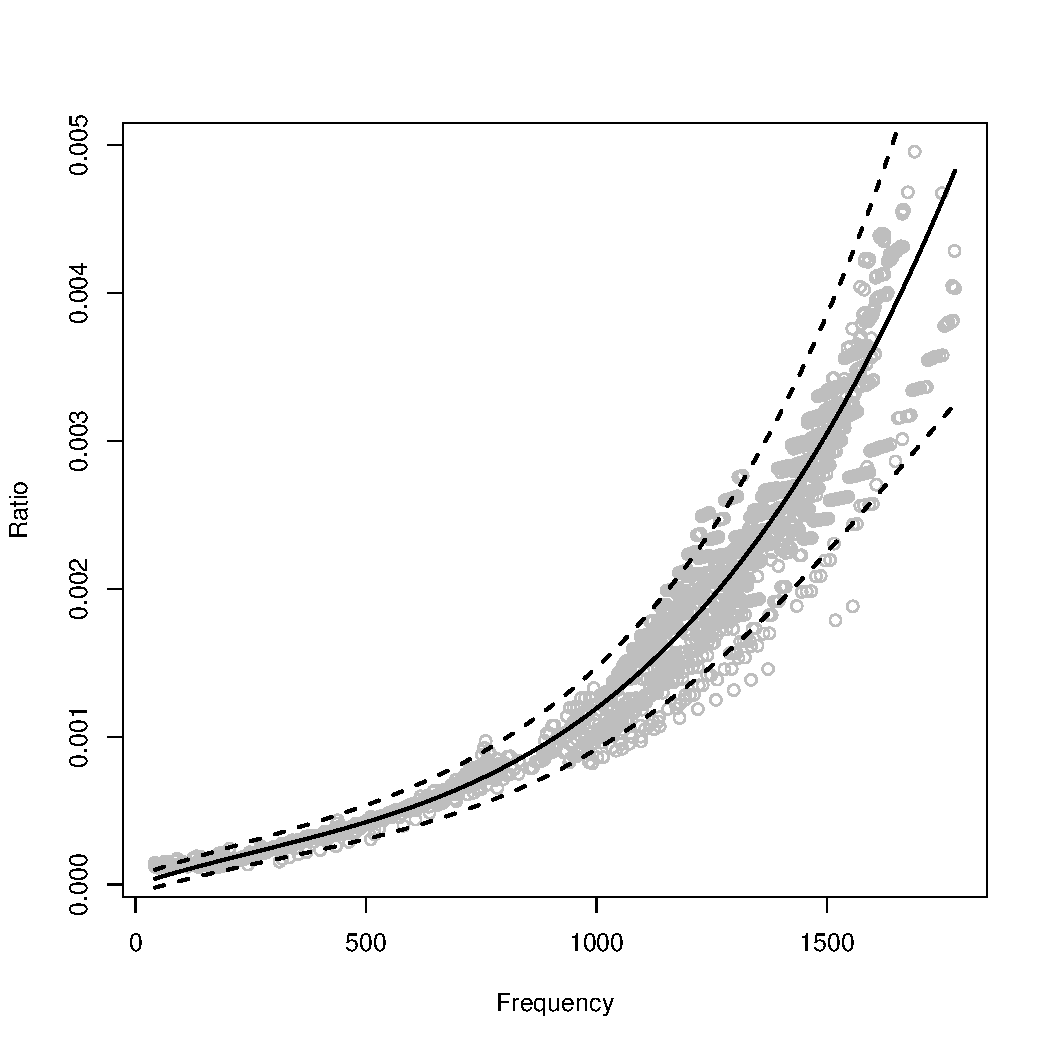
\includegraphics[width=0.5\textwidth]{plots/model}
 \caption{Ratio $M_{\rm PNS}/R_{\rm PNS}^2$ from 25 1D simulations {\sc AENUS-ALCAR} (red) and {\sc CoCoNuT} (green) code. The solid line is the maximum likelihood estimate of heteroscedastic cubic model with 95\% confidence bands (dashed lines) considering \pcd{only} the  {\sc AENUS-ALCAR} data points \pcd{($18$ simulations)}. \mab{To be redone in python}} \label{fig:LMVAR}
\end{figure}

{We use this model to infer the properties of the simulations in the 
{\it test set} described in in Section \ref{sec:simulations}.}
To describe the method we focus on the GW signal
of {\texttt s20S}, originally
sampled at 16384 Hz but resampled at 4096 Hz.
A spectrogram of this signal is shown in Figure \ref{fig:spectrogram} based on
autoregressive estimates \pcd{[add ref?]}of the local spectra for successive time intervals of 
\textcolor{red}{length 200} with a \textcolor{red}{ 90\%} overlap.
The dominant emission mode corresponds to the PNS oscillation $\mbox{}^2 g_2$-mode. We have
developed a time-frequency method to track the ridge $m(t) $in the spectrogram,
taking into account that it is monotonically increasing as time goes. 
{This is a property of the $\mbox{}^2 g_2$-mode, the frequency of which  
increases as the object becomes more massive and compact}.
Starting from either the left- or right-most column of the time-frequency matrix
we identify and trace the sequence of amplitude peaks within a certain frequency
band given the monotonicity constraint. Appendix \ref{app:gmode} is providing more
details on the reconstruction of the $g$ mode ridge. 


\begin{figure}
 \centering
 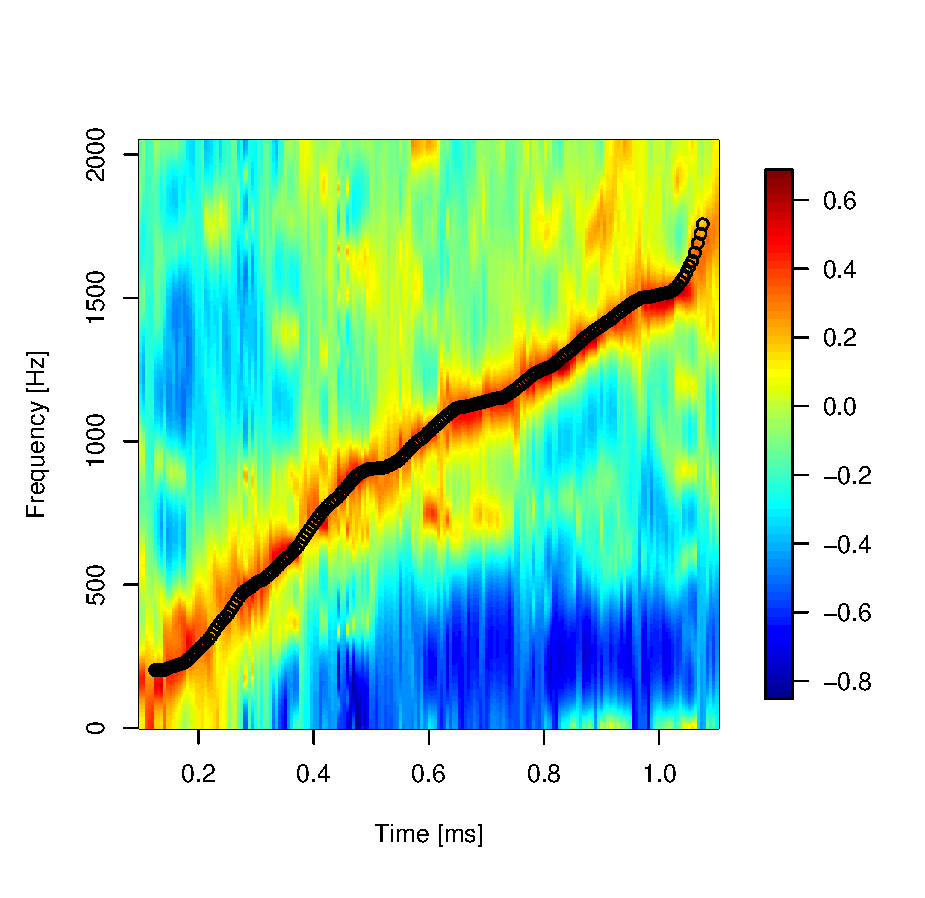
\includegraphics[width=0.5\textwidth,height=0.3\textheight]{plots/spectrogram}
 \caption{Spectrogram of the GW signal {\texttt s20S} sampled at \unit[4096]{Hz}.
   The spectrogram is obtained using data streach of 200 samples overlapping at 90\%
   with each other. \mab{To be redone in python}} \label{fig:spectrogram}
\end{figure}

We collect the instantaneous frequency $f(t_i)$ corresponding to the ridge $m(t_i)$ for
the midpoint $t_i$ of each local time interval of the spectrogram and interpolating $f(t)$
for values in between the $t_i$. We then use our model given by Eq.~\eqref{eq:model1} to obtain
estimates of the time evolution of the ratio together with 95\% confidence intervals.
An example is given in Figure \ref{fig:ratio} where the red points are the point estimates and
the grey bands represent 95\% confidence bands. Ratio values
computed using the mass and radius values obtained from the simulation code \pcd{(true values)}
are shown in black.
In this example of a GW signal without noise the coverage of our 95\% confidence band is 100\%
of the true values.
In the next section we investigate the performance of the reconstruction of $r(t)$ when the GW
signal is embedded in noise.

\begin{figure}
 \centering
 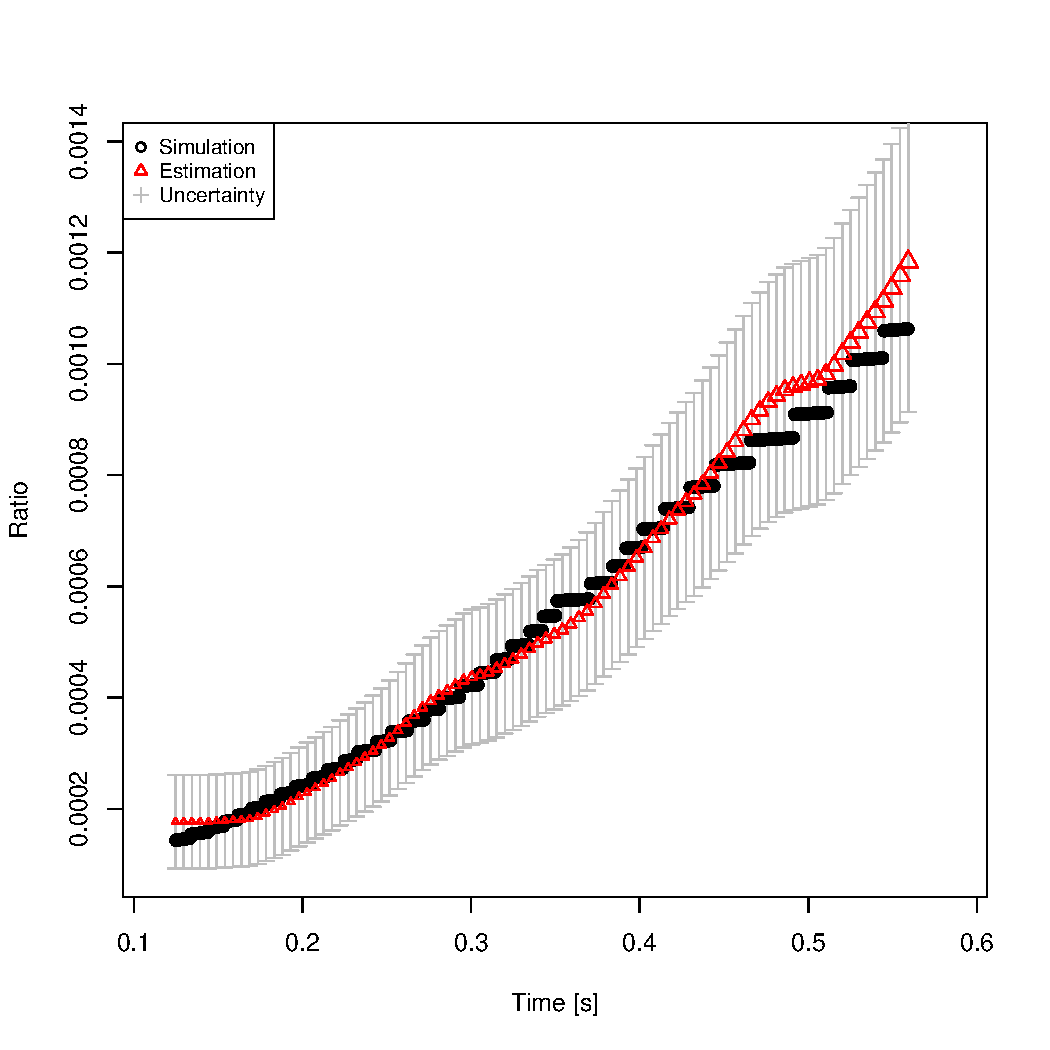
\includegraphics[width=0.5\textwidth,height=0.3\textheight]{plots/ratio}
 \caption{Ratio $M_{\rm PNS}/R_{\rm PNS}^2$ as function of time extracted from the $\mbox{}^2 g_2$-mode of the {\texttt s20S} signal (red points and the 95\% confidence belt in grey) compared to the ratio value derived from the PNS mass and radius given by the simulation code (black points) \mab{To be redone in python}.} \label{fig:ratio}
\end{figure}


